\chapter{Moving spiral wave chimeras (Physical Review E, 104(2), L022203)}

So far, we have devoted our investigation to one-dimensional localized states
that forcefully drift due to a symmetry-breaking term. In contrast, in this
second half of the dissertation, we present and analyze a two-dimensional 
localized state where the motion arises spontaneously.

Coupled oscillators, synchronization. Very important in many contexts, brain, heart,
electrical grid, etc.

Unexpectedly, a different state was also found: the chimera state. explain
They have been predicted and experimentally observed in a plethora of systems
[refs]. 

In the weak coupling limit, these populations of nonlinear oscillators can be accurately
described by a simple yet powerful model: the Kuramoto model. 


This second half will be devoted to the study of coupled phase oscillators. As
stated previously, in section~\ref{sec:phase_oscillators}, the dynamics of
a non-linear oscillator, in the limit of weak coupling, can be reduced
to a single cyclic variable: the phase. Therefore, an adequate and general model
for a population of coupled oscillators  

[synchronization in the brain] \cite{erra2017neuralsynchronization}

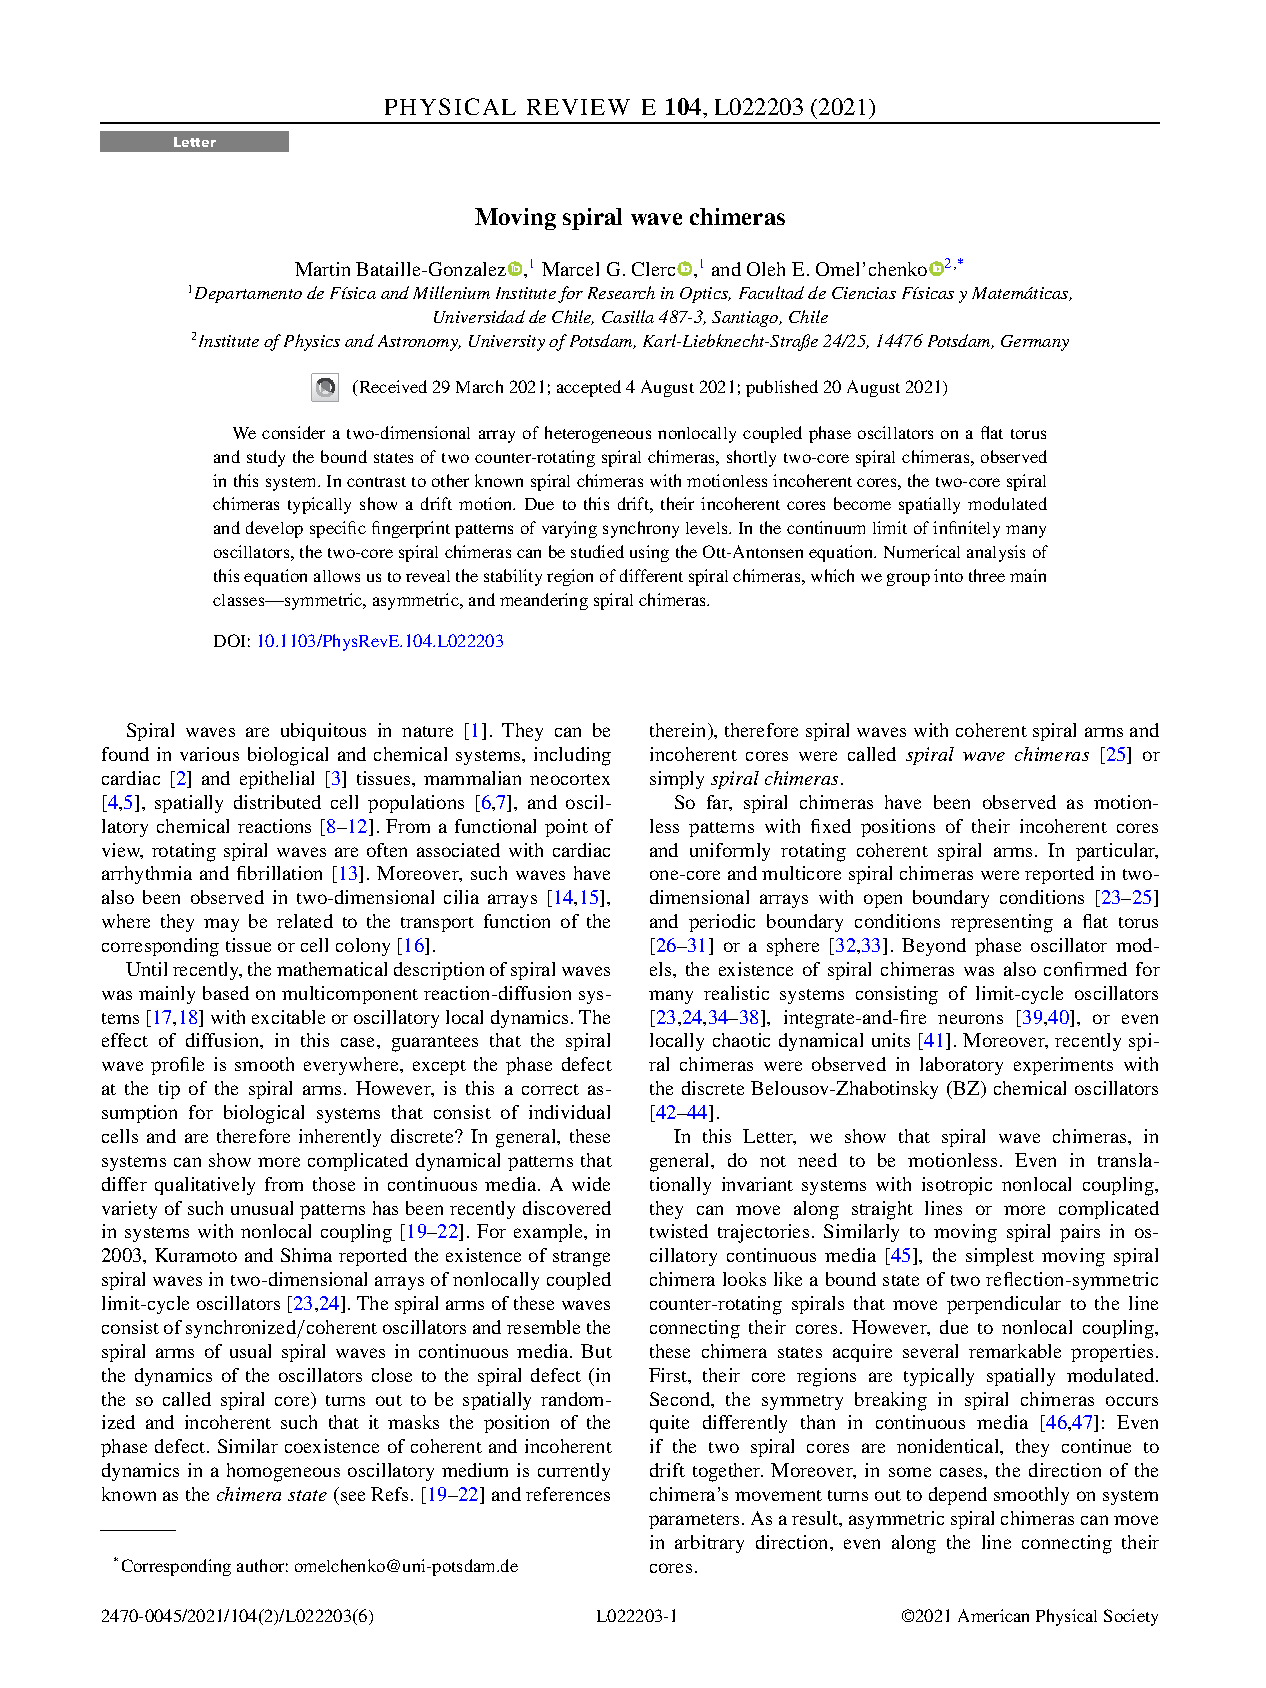
\includepdf[pages={-}]{chapters/movingspirals.pdf}
